\documentclass[12pt]{article}

\usepackage{graphicx}
\usepackage[a4paper,margin=1in]{geometry}
\usepackage{amsmath,amssymb}
\usepackage{textcomp}

\begin{document}

\noindent
\begin{minipage}{0.38\textwidth}

\textbf{KUNE PAVITHRA}

\vspace{0.2cm}

\textbf{COMET FWC 69}

\end{minipage}
\begin{minipage}{0.6\textwidth}

\begin{flushright}

\includegraphics[width=0.75\textwidth]{IIITB_logo_with_Institute_Name_jpeg1.jpg}
\end{flushright}

\end{minipage}

\vspace{0.5cm}

\begin{center}

{\fontsize{22}{24}\selectfont
\textbf{Mathematics Olympiad Task}
}

\end{center}

\section*{Q14}

In fig. 6, find the area of the shaded region enclosed between two concentric circles of radii 7 cm and 14 cm where $\angle AOC = 40^\circ$.

Use $\pi = \frac{22}{7}$.

\begin{center}
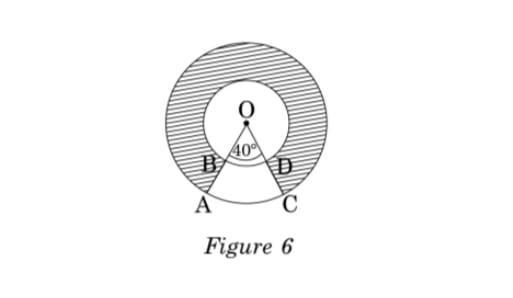
\includegraphics[width=0.45\textwidth]{figure6.jpg}
\end{center}

\section*{Q15}

If the ratio of the sum of first $n$ terms of two A.P's is

\begin{align*}
(7n+1):(4n+27)
\end{align*}

find the ratio of their $m$th terms.

\section*{Q16}

Solve for $x$:

\begin{align*}
\frac{1}{(x-1)(x-2)}
+
\frac{1}{(x-2)(x-3)}
=
\frac{2}{3}
\end{align*}

where $x \neq 1,2,3$.

\section*{Q17}

A conical vessel with base radius 5 cm and height 24 cm is full of water. This water is emptied into a cylindrical vessel of base radius 10 cm.

Find the height to which the water rises.

\section*{Q18}

A sphere of diameter 12 cm is dropped into a cylindrical vessel partly filled with water. The water level rises by 32 cm.

Find the diameter of the cylindrical vessel.

\section*{Q19}

A man standing on the deck of a ship 10 m above water level observes the angle of elevation of the top of a hill as $60^\circ$ and angle of depression of the base of hill as $30^\circ$.

Find:

\begin{itemize}

\item Distance of hill from ship

\item Height of hill

\end{itemize}

\section*{Q20}

Three different coins are tossed together.

Find the probability of getting:

\begin{itemize}

\item exactly two heads

\item at least two heads

\item at least two tails

\end{itemize}

\section*{Q21}

Due to heavy floods in a state, thousands were rendered homeless. 50 schools collectively offered place and canvas for 1500 tents.

Each tent has:

\begin{itemize}

\item cylindrical base of radius 2.8 m and height 3.5 m

\item conical top of radius 2.8 m and height 2.1 m

\end{itemize}

If canvas costs Rs.120 per sq.m, find the amount shared by each school.

What value is generated by this problem?

\section*{Q22}

Prove that the lengths of tangents drawn from an external point to a circle are equal.

\section*{Q23}

Draw a circle of radius 4 cm. Draw two tangents to the circle inclined at an angle of $60^\circ$ to each other.

\section*{Q24}

In Fig. 7, two equal circles with centres O and O' touch each other at X.

$OO'$ produced meets the circle with centre O' at A.

AC is tangent to the circle with centre O at C.

$O'D \perp AC$.

Find:

\begin{align*}
\frac{CO}{DO'}
\end{align*}

\begin{center}
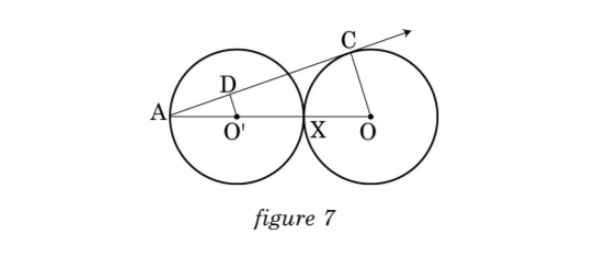
\includegraphics[width=0.45\textwidth]{figure7.jpg}
\end{center}

\section*{Q25}

Solve for $x$:

\begin{align*}
\frac{1}{x+1}
+
\frac{1}{x+2}
+
\frac{1}{x+4}
=
\frac{2}{x}
\end{align*}

where $x \neq -1,-2,-4$.

\section*{Q26}

The angle of elevation of the top Q of a vertical tower PQ from a point X on the ground is $60^\circ$.

From a point Y, 40 m vertically above X, the angle of elevation of the top Q of tower is $45^\circ$.

Find:

\begin{itemize}

\item height of tower PQ

\item distance PX

\end{itemize}

Use $\sqrt{3}=1.73$.

\vspace{0.7cm}

\textbf{Prove the following:}

\begin{enumerate}

\item

\begin{align*}
3\sin^{-1}x
=
\sin^{-1}(3x-4x^3),
\quad
x \in \left[-\frac{1}{2},\frac{1}{2}\right]
\end{align*}

\item

\begin{align*}
3\cos^{-1}x
=
\cos^{-1}(4x^3-3x),
\quad
x \in \left[\frac{1}{2},1\right]
\end{align*}

\item

\begin{align*}
\tan^{-1}\frac{2}{11}
+
\tan^{-1}\frac{7}{24}
=
\tan^{-1}\frac{1}{2}
\end{align*}

\item

\begin{align*}
2\tan^{-1}\frac{1}{2}
+
\tan^{-1}\frac{1}{7}
=
\tan^{-1}\frac{31}{17}
\end{align*}

\end{enumerate}

\vspace{0.5cm}

\textbf{Write the following functions in the simplest form:}

\begin{enumerate}

\item[5.]

\begin{align*}
\tan^{-1}
\left(
\frac{\sqrt{1+x^2}-1}{x}
\right),
\quad x \neq 0
\end{align*}

\item[6.]

\begin{align*}
\tan^{-1}
\left(
\frac{1}{\sqrt{x^2-1}}
\right),
\quad |x|>1
\end{align*}

\item[7.]

\begin{align*}
\tan^{-1}
\left(
\sqrt{
\frac{1-\cos x}{1+\cos x}
}
\right),
\quad 0<x<\pi
\end{align*}

\item[8.]

\begin{align*}
\tan^{-1}
\left(
\frac{\cos x-\sin x}
{\cos x+\sin x}
\right),
\quad
-\frac{\pi}{4}
<
x
<
\frac{3\pi}{4}
\end{align*}

\item[9.]

\begin{align*}
\tan^{-1}
\left(
\frac{x}{\sqrt{a^2-x^2}}
\right),
\quad |x|<a
\end{align*}

\item[10.]

\begin{align*}
\tan^{-1}
\left(
\frac{3a^2x-x^3}
{a^3-3ax^2}
\right)
\end{align*}

\begin{align*}
a>0,
\quad
-\frac{a}{\sqrt{3}}
<
x
<
\frac{a}{\sqrt{3}}
\end{align*}

\end{enumerate}

\vspace{0.5cm}

\textbf{Find the values of each of the following:}

\begin{enumerate}

\item[11.]

\begin{align*}
\tan^{-1}
\left[
2\cos
\left(
2\sin^{-1}\frac{1}{2}
\right)
\right]
\end{align*}

\item[12.]

\begin{align*}
\sin
\left(
\sin^{-1}\frac{1}{5}
+
\cos^{-1}x
\right)
=
1
\end{align*}

Find $x$.

\end{enumerate}

\end{document}
